TODO add the second training loss for the second autoencoder
\begin{figure}[htb]
	\begin{center}
		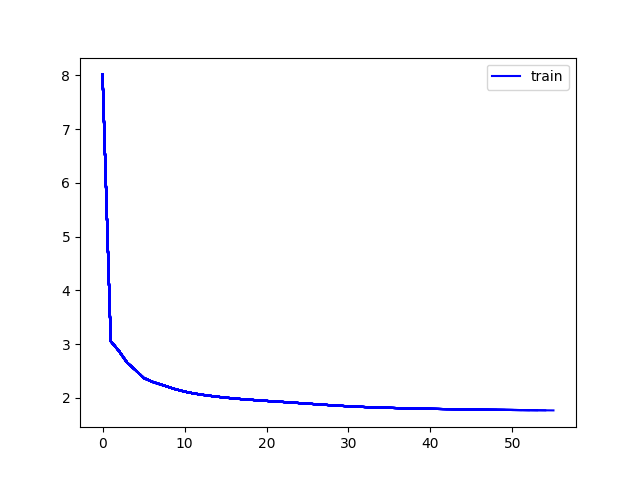
\includegraphics[width=0.5\linewidth]{bilder/ae-embeddings/training-ae-.png}
		\caption{Autoencoder training convergence}\label{fig:ae-training}
	\end{center}
\end{figure}

\begin{figure}[htb]
	\begin{center}
		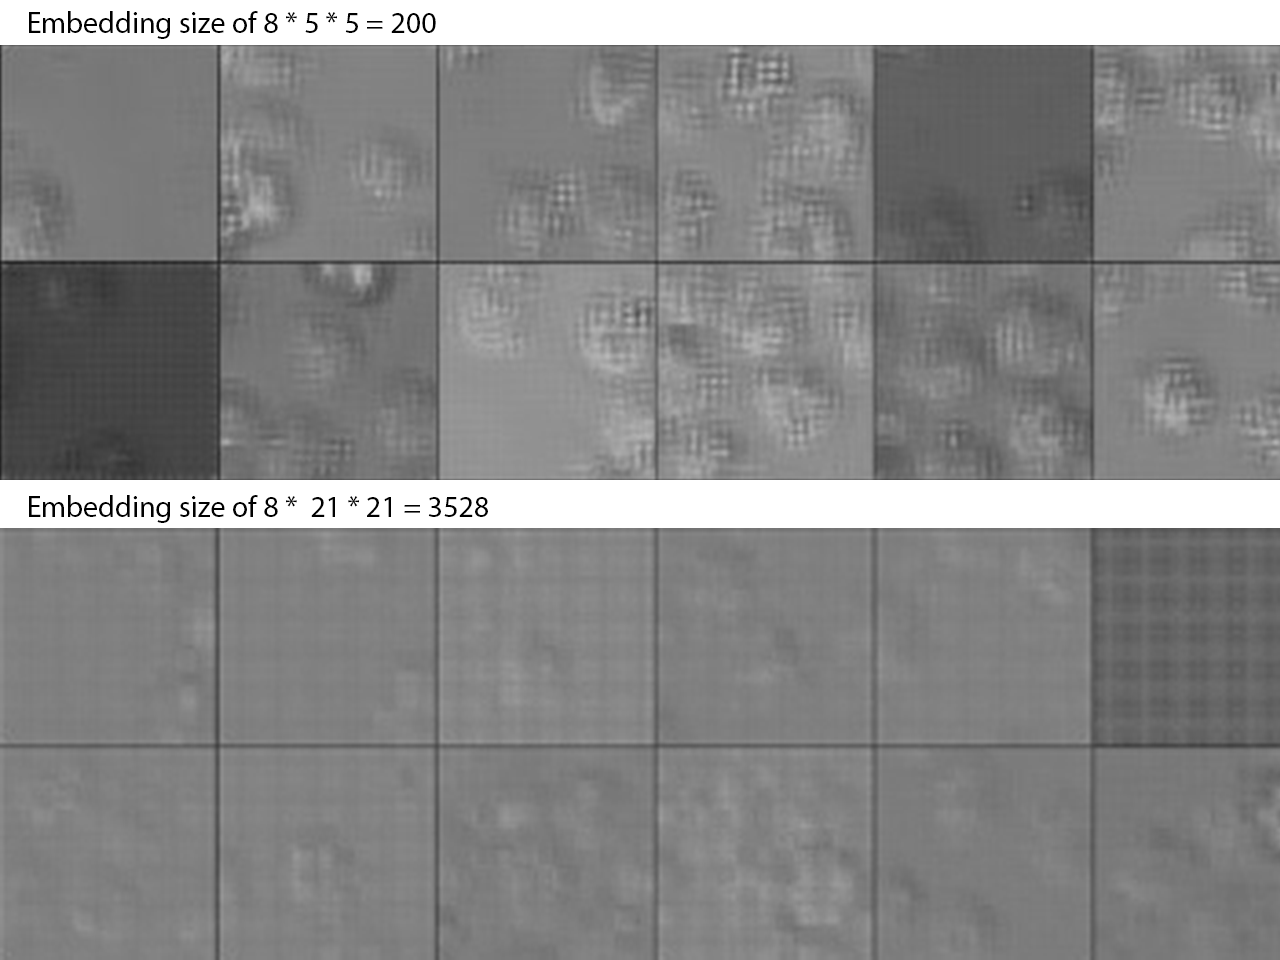
\includegraphics[width=0.5\linewidth]{bilder/ae-embeddings/ae-samples.png}
		\caption{Samples drawn from the trained autoencoder}\label{fig:ae-samples}
	\end{center}
\end{figure}

\begin{figure}[htb]
	\begin{center}
		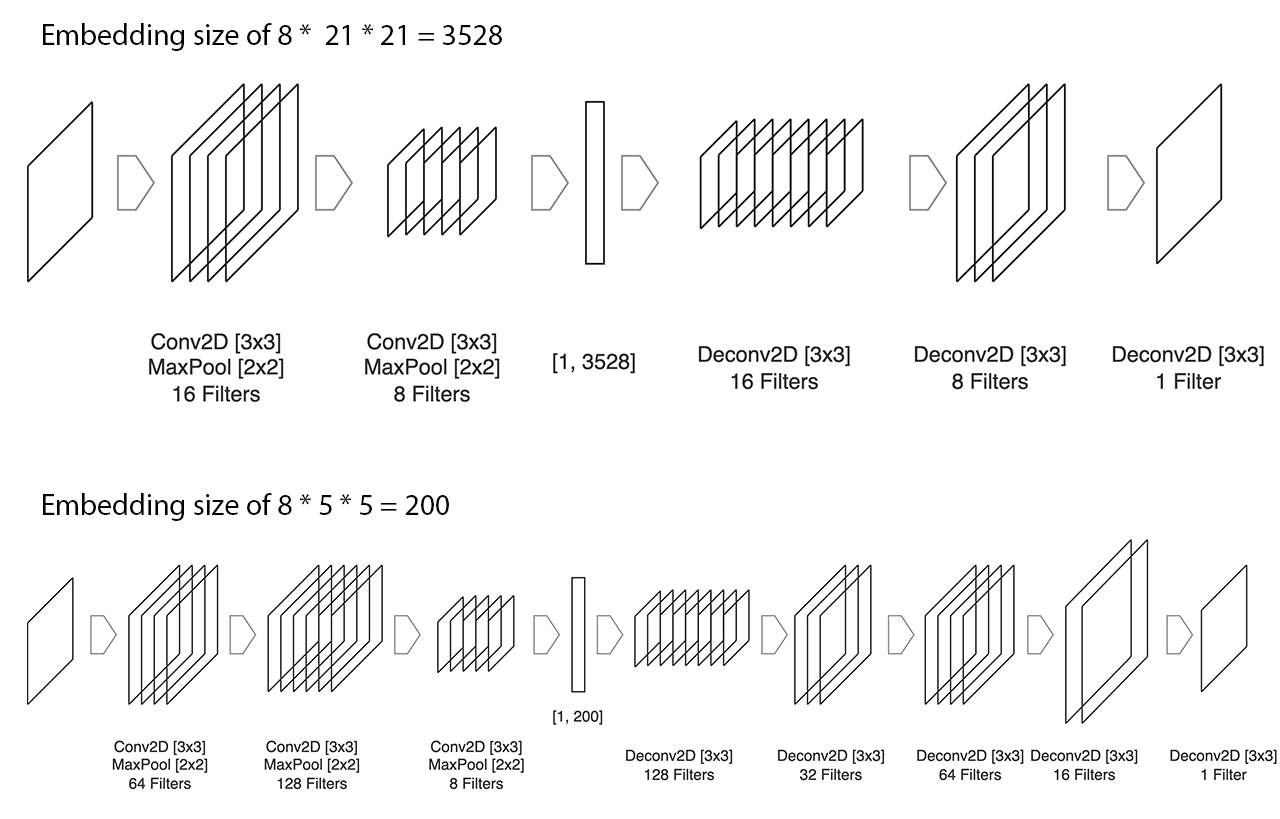
\includegraphics[width=0.5\linewidth]{bilder/ae-embeddings/ae-architecture.png}
		\caption{Architectures of two autoencoders}\label{fig:ae-architecture}
	\end{center}
\end{figure}

\begin{figure}[htb]
	\begin{center}
		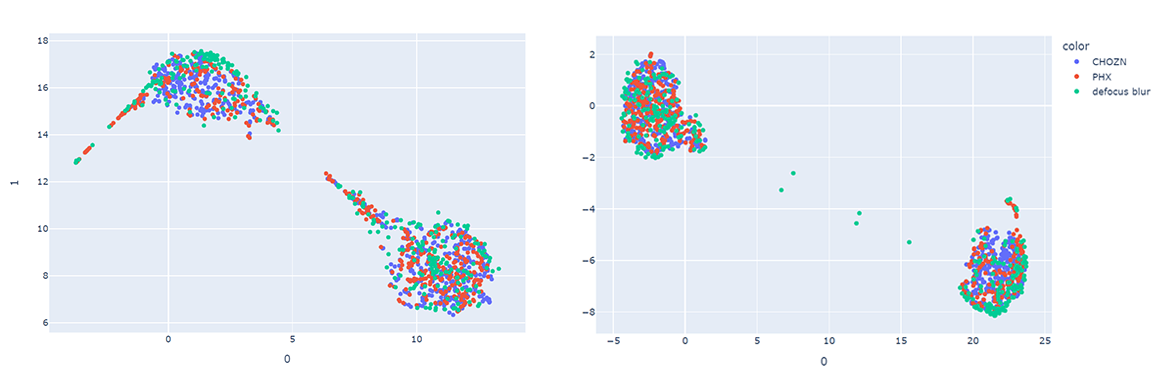
\includegraphics[width=0.5\linewidth]{bilder/ae-embeddings/pca-umap-clusters.png}
		\caption{Autoencoder embeddings after applying PCA with 10 components and UMAP afterwards. Earlier epoch VS later epoch}\label{fig:ae-pca-umap-clustered}
	\end{center}
\end{figure}

\begin{figure}[htb]
	\begin{center}
		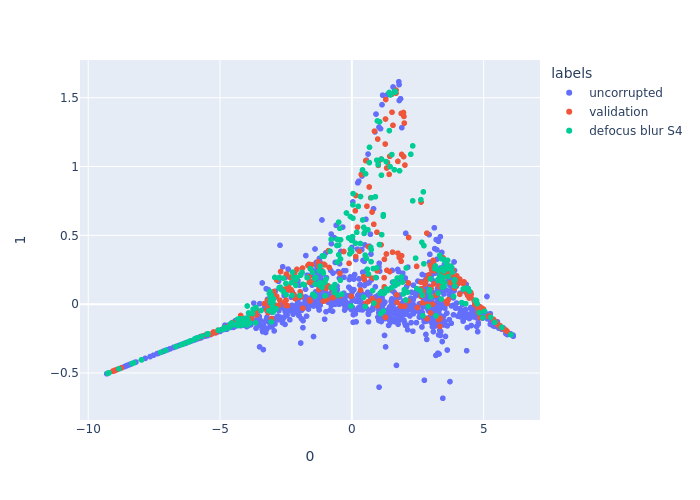
\includegraphics[width=0.5\linewidth]{bilder/ae-embeddings/pacmap.png}
		\caption{PacMAP does not provide information on the coruption}\label{fig:ae-pacmap}
	\end{center}
\end{figure}

\begin{figure}[htb]
	\begin{center}
		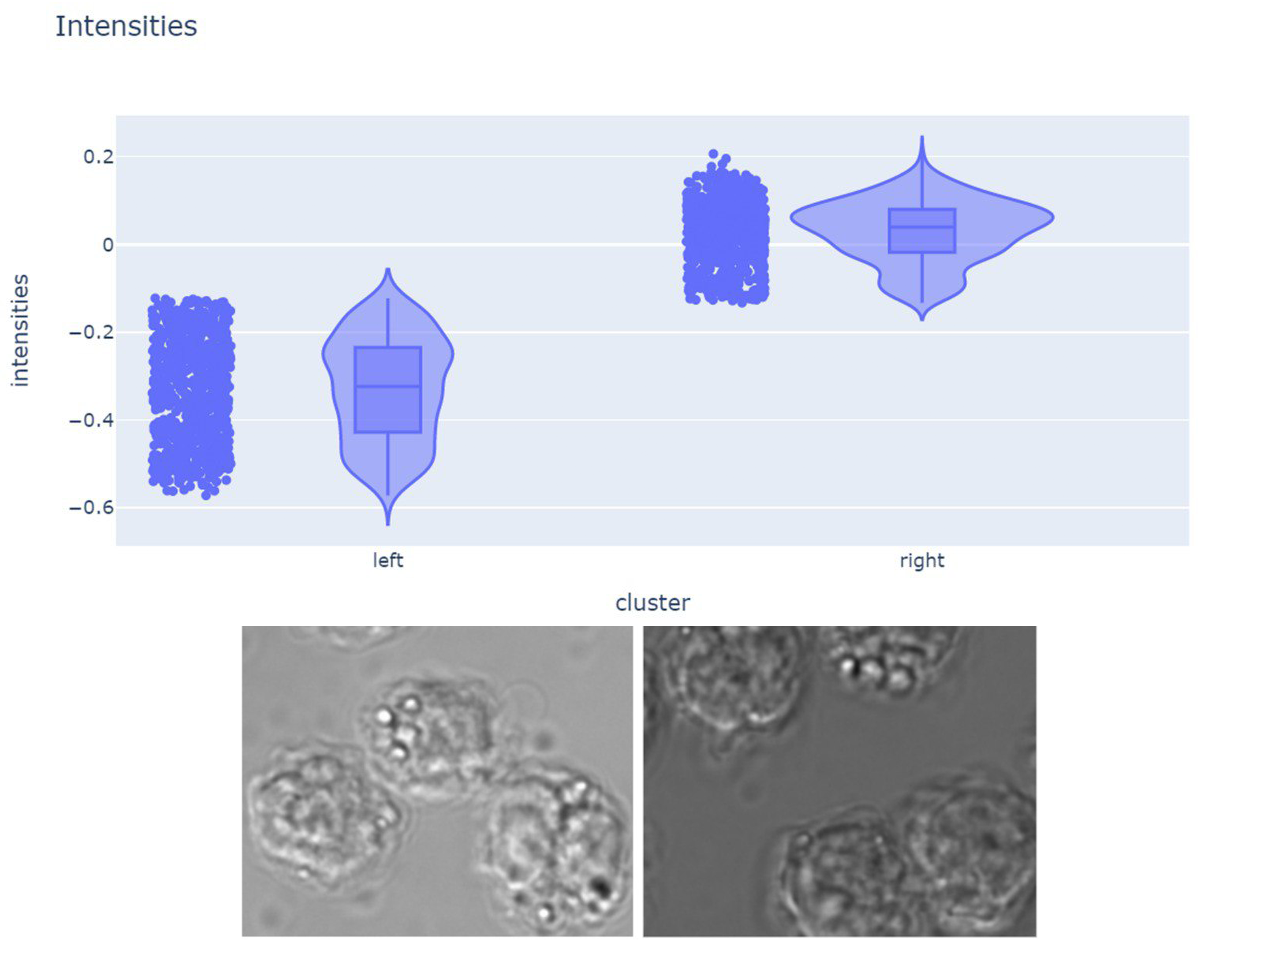
\includegraphics[width=0.5\linewidth]{bilder/ae-embeddings/brighter-darker.png}
		\caption{What do two UMAP clusters represent}\label{fig:ae-brighter-darker}
	\end{center}
\end{figure}



